\documentclass[margin,line]{res}
\usepackage{hyperref}
\usepackage{url}
\usepackage{graphicx}
\oddsidemargin -.5in
\evensidemargin -.5in
\textwidth=6.0in
\itemsep=0in
\parsep=0in
\topmargin=0in
\topskip=0in
 
\newenvironment{list1}{
  \begin{list}{\ding{113}}{%
      \setlength{\itemsep}{0in}
      \setlength{\parsep}{0in} \setlength{\parskip}{0in}
      \setlength{\topsep}{0in} \setlength{\partopsep}{0in}
      \setlength{\leftmargin}{0.17in}}}{\end{list}}
\newenvironment{list2}{
  \begin{list}{$\bullet$}{%
      \setlength{\itemsep}{0in}
      \setlength{\parsep}{0in} \setlength{\parskip}{0in}
      \setlength{\topsep}{0in} \setlength{\partopsep}{0in}
      \setlength{\leftmargin}{0.2in}}}{\end{list}}


    
\begin{document}

\name{\LARGE NIKHILESH MATH} \hfill {\em \today}

\begin{resume}
\section{\sc Contact Information}

\vspace{.05in}
\begin{tabular}{@{}p{3.5in}p{3in}}
\#241,5th main road,             & {Phone:}  +91 7676301776 \\
3rd Block Thyagaraja Nagar 
 & {E-mail:}  nikhileshm9@gmail.com\\
Bengaluru - 560028.\\
 & 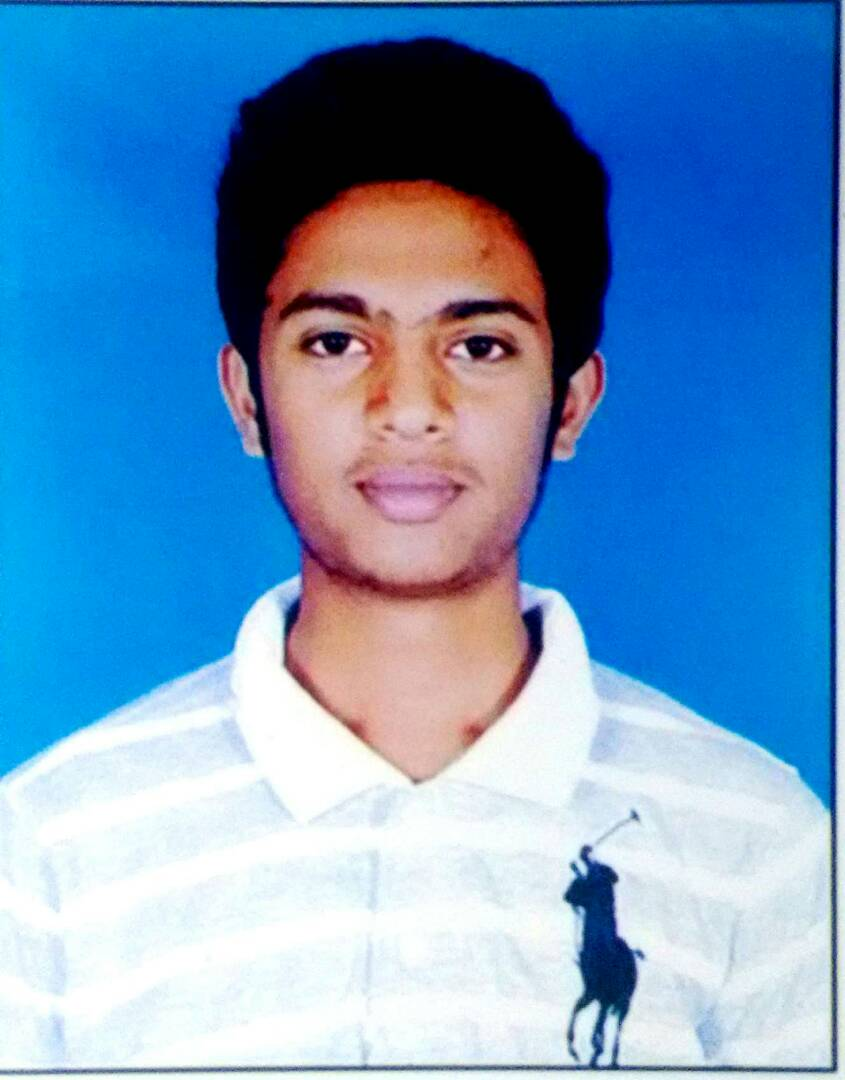
\includegraphics[width=5cm]{PassportPhoto}
\end{tabular}
\section{\sc Objective}

Seeking an internship position as a part of eYSIP - 2017 at Indian Institute of Technology,Bombay to explore career options in the Embedded Research Sector . A hard-working and self-motivated undergraduate student in 3rd year Electronics and Communication.

\section{\sc Education}
\begin{tabular}{ L{1in} L{1in} L{1in} L{0.5in} L{1in} }
	\textbf{Degree} & \textbf{College/School} & \textbf{University} & \textbf{Passing Year} & \textbf{Pass Percentage} \\ 
	\hline \\
	B.E(ECE) & B.M.S College & Visvesvaraya  & 2018 & 8.32 (As of Sem V) \\ &  of Engineering & Technological University & & \\ \\
	12th & Independent & Department of Pre-University & 2014 & 87\% \\ & PU College & Education, Karnataka & & \\
	10th & Nandi International& Central Board of & 2012 & 8.6 \\ &  School,Bellary & Secondary Education & & \\
	\hline	
\end{tabular}

\section{\sc Projects}
\begin{enumerate}
	\item \textbf{Wireless Joystick Controller} using mbed1768 ARM Cortex M3 Based Microcontroller , xbee module and USB HID.
	\item \textbf{Two-wheeled Self Balancing Robot} using ATMega 2560 as part of E-Yantra Robotics Competition, 2016-17.
	\item \textbf{OCR Puzzle Solving Robot} based on the Firebird V Platform as part of E-Yantra Robotics Competition, 2015-16.
	\item \textbf{OCR Puzzle Solving Robot} based on the Firebird V 8051 Platform as part of 8051 Microcontroller Application, 2015-16.	
	\item Object Detection using Google API platform.
	\item \textbf{6T S-RAM Cell} with Cadence tool.		    
\end{enumerate}

\section{\sc Training And Internship}
\begin{itemize}
	\item Java SE
	\item Oracle
\end{itemize}

\section{\sc Research and Publications}
N.A\\

\section{\sc Technical Skills}
\begin{itemize}
	\item Programming Languages - Java SE, C, C++, Python, MATLAB, Embedded C, Oracle , Basic HTML, Basic Android Application Devolopment.
	\item VLSI Design - Verilog HDL, Cadence Virtuoso.
	\item Microcontrollers - Intel 8051, AVR ATMega Microcontrollers, Arduino, ARM Cortex M3 Based mbed Series Microcontrollers.
	\item Technical Writing - Microsoft Word, Microsoft Excel, Microsoft Powerpoint, LaTeX.
	\item Image Processing - Matlab, Python.
\end{itemize}

\section{\sc Soft Skills}


\begin{enumerate}
	\item Able to Listen
	\item Accept Feedback
	\item Adaptable
	\item communication skills
	\item information collection and management
	\item organizing and planning skills
	\item problem-solving
	\item creativity
	\item persuasiveness
	\item initiative		    
\end{enumerate}

\section{\sc Extra Curricular Activities}
\begin{itemize}
	\item online courses from edx and coursera.
\end{itemize}

\section{\sc Co Curricular Activities}
\begin{enumerate}
	\item Participated and Won in Self Balancing Robot Theme of E-Yantra Robotics Competition,2016-17.
	\item Participated and Progressed to task 2 in Puzzle Solver Theme of E-Yantra Robotics Competition,2016-17.	    
\end{enumerate}

\section{\sc Personal Information}
Father's Name : Chandra Mouli M\\
Mother's Name : Vanajamma\\
Sex : Male\\
Date of Birth : 13th Sept,1996\\
Nationality : Indian\\
Marital Status : Unmarried\\

\section{\sc References}
Furnished upon request.\\

\section{\sc Declaration}
I do hereby declare that the above given information is true and correct to the best of my knowledge.\\

\end{resume}
\end{document}




